\documentclass{beamer}
\usepackage[latin1]{inputenc,colortbl}
\usepackage{epsfig}
\usetheme{Frankfurt}
\setbeamertemplate{navigation symbols}{}
\setbeamertemplate{footline}[page number]
%\newtheorem{definition}{Definition}
\title[Analyzing the Interaction between Knowledge and Social Commitment in Multi-Agent Systems]{Analyzing the Interaction between Knowledge and Social Commitments in Multi-Agent Systems}
\author{Faisal Al-Saqqar\\ \vspace{0.2cm} Supervised by: Dr. Jamal Bentahar}
\institute{Department of Computer Science and Software Engineering\\Concordia University}
\date{August 08, 2013}
\begin{document}
%%%%%%%%%%%%%%%%%%%%%%%%%%%%%%%% frame1 title page %%%%%%%%%%%%%%%%%%%%%%%%%%%%%%%%%%%%%%%
%%%%%%%%%%%%%%%%%%%%%%%%%%%%%%%%%%%%%%%%%%%%%%%%%%%%%%%%%%%%%%%%%%%%%%%%%%%%%%
\begin{frame}
\titlepage
\end{frame}
%%%%%%%%%%%%%%%%%%%%%%%%%%%%%%%% frame2 outline page %%%%%%%%%%%%%%%%%%%%%%%%%%%%%%%%%%%%%
%%%%%%%%%%%%%%%%%%%%%%%%%%%%%%%%%%%%%%%%%%%%%%%%%%%%%%%%%%%%%%%%%%%%%%%%%%%%%%

\begin{frame}{Presentation Outline}
    \begin{itemize}
     	\itemsep=.5cm
    	\item {\bf Introduction}
    	\item Background and Literature Review
    	\item Proposed Research
        \item Contributions and Research Activities
    	\item Time Line
    \end{itemize}
\end{frame}

%%%%%%%%%%%%%%%%%%%%%%%%%%%%%%%% frame3 introduction %%%%%%%%%%%%%%%%%%%%%%%%%%%%%%%%%%%%%
%%%%%%%%%%%%%%%%%%%%%%%%%%%%%%%%%%%%%%%%%%%%%%%%%%%%%%%%%%%%%%%%%%%%%%%%%%%%%%
\section{Introduction}
%\section{Motivation}
\subsection{Multi-Agent Systems MASs}
    \begin{frame}{Motivation}
    \begin{itemize}
    \item In concrete applications such as business settings, agents should reason on their knowledge and their social commitments at the same time, particularly when they are engaged in conversations.
    \item Examples:
     \begin{itemize}
      \item \textbf{NetBill payment protocol}.
      \item \textbf{The travel agent}.
      \item \textbf{The car rental company}.
     \end{itemize}
\end{itemize}
\begin{figure}[htbp]
\centering
%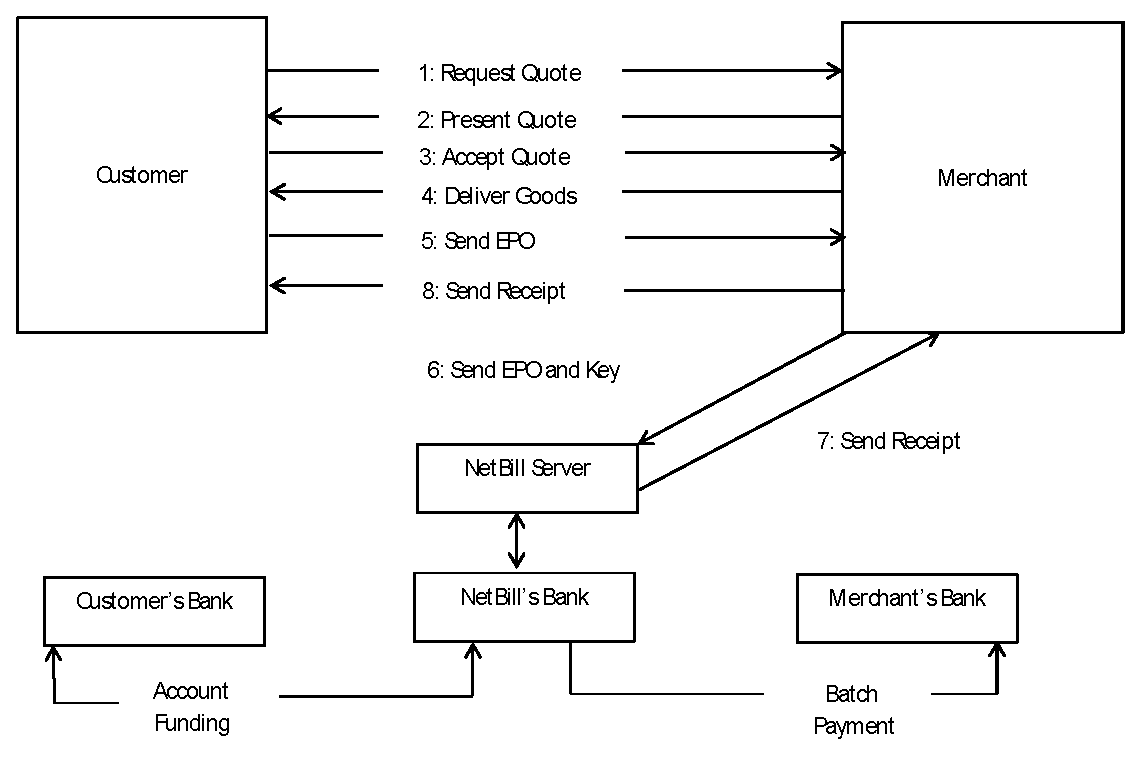
\includegraphics[width=12cm, height=8cm]{figures/figure1.eps}
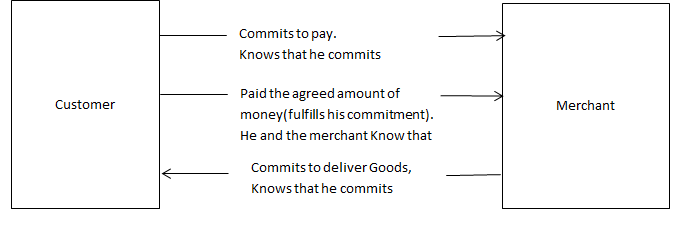
\includegraphics[width=1.0 \columnwidth]{figures/figure7.png}
%%\includegraphics[scale=0.5]{figure1}
%\caption{The NetBill payment protocol} \label{figure7}
\end{figure}
    \end{frame}
%%%%%%%%%%%%%%%%%%%%%%%%%%%%%%%%%%%%%%%%%%%%%%%%%%%%%%%%%%%%%%%%%%%%%%%%%%%%%%
\begin{frame}{Problems and Research Questions}

\begin{itemize}
\item \textbf{How to analyze the interaction between knowledge and social commitments in MASs?}.
\item There is \textbf{no formal framework and semantics} available in the
literature that allow us to reason about knowledge and social commitments in MASs at the same time.


\end{itemize}

\end{frame}
%%%%%%%%%%%%%%%%%%%%%%%%%%%%%%%%%%%%%%%%%%%%%%%%%%%%%%%%%%%%%%%%%%%%%%%%%%%%%%

\begin{frame}{Continue: Problems and Research Questions}
 \begin{itemize}
   \item \textbf{How can we define a formal computational logic that can capture both knowledge and social commitments, so that properties involving both of them simultaneously can be expressed?}
        \begin{itemize}
         \item Combining logics of knowledge and commitments into one logic called Computation Tree Logic of Knowledge and Commitments (CTLKC).
        \end{itemize}
    \item \textbf{Is it enough to simply combine the current versions of knowledge and commitment logics?}
        \begin{itemize}
         \item Analyze the consistency of the CTLKC logic.
        \end{itemize}
    \item \textbf{What are the characteristics of the new logic that will combine knowledge and commitments?}
        \begin{itemize}
         \item The new logic should solve any inconsistency that might result from the combination of the two logics.
        \end{itemize}
\end{itemize}
\end{frame}
%%%%%%%%%%%%%%%%%%%%%%%%%%%%%%%%%%%%%%%%%%%%%%%%%%%%%%%%%%%%%%%%%%%%%%%%%%%%%%%
%    \begin{frame}{Multi-Agent Systems MASs}
%        \begin{itemize}
%            \itemsep=.35cm
%        	\item Multi-Agent System (MAS).
%            %\item Autonomous agents.
%        	\item Knowledge in MASs.
%            \item Social commitments in MASs.
%        \end{itemize}
%\end{frame}

%%%%%%%%%%%%%%%%%%%%%%%%%%%%%%%%%%%%%%%%%%%%%%%%%%%%%%%%%%%%%%%%%%%%%%%%%%%%%%
\section{Background}
\begin{frame}{Presentation Outline}
    \begin{itemize}
     	\itemsep=.5cm
    	\item Introduction
    	\item {\bf Background and Literature Review}
    	\item Proposed Research
        \item Contributions and Research Activities
    	\item Time Line
    \end{itemize}
\end{frame}

%%%%%%%%%%%%%%%%%%%%%%%%%%%%%%%% frame9 Background and Literature Review %%%%%%%%%%%%%%%%%%%%%%%%%%%%%%%%%%%%%
%%%%%%%%%%%%%%%%%%%%%%%%%%%%%%%%%%%%%%%%%%%%%%%%%%%%%%%%%%%%%%%%%%%%%%%%%%%%%%
\subsection{Knowledge in MASs}
    \begin{frame}{Knowledge in MASs}

        \begin{itemize}
            \itemsep=.35cm
        	\item \textbf{Knowledge in MASs}.

             \begin{itemize}
              \item Hintikka and Lenzen.
              \item Kripke Models $M = (S, \{R_i\}_{i \in A}, V)$.
              \item Interpreted Systems.\\
              The formalism of interpreted systems is used to model the temporal evolution of a system of agents in order to reason about knowledge and temporal properties.\\
\textbf{Example:} ``Bob knows that it is sunny in Montreal".\\
This knowledge is denoted by $K_{Bob} \varphi$, where $\varphi$ means it is sunny in Montreal.
            \end{itemize}
        	      	
        \end{itemize}


    \end{frame}
%%%%%%%%%%%%%%%%%%%%%%%%%%%%%%%% frame10 Background and Literature Review %%%%%%%%%%%%%%%%%%%%%%%%%%%%%%%%%%%%%
%%%%%%%%%%%%%%%%%%%%%%%%%%%%%%%%%%%%%%%%%%%%%%%%%%%%%%%%%%%%%%%%%%%%%%%%%%%%%%
\subsection{Social commitments in MASs}
    \begin{frame}{Commitments in MASs}
        Agent Communication Languages (ACLs).
        \begin{itemize}
            \itemsep=.35cm
        	\item \textbf{Commitments in MASs}
            \begin{itemize}
              \item \textbf{Mental Approaches}. \\Agents can read each other minds.
              \item \textbf{Social Approaches}. \\
              Formally, $C_{i\rightarrow j}\varphi$ means that agent $i$, the debtor (that makes the commitment), commits to agent $j$, the creditor (towards which the commitment is made), that $\varphi$ (the content of the commitment) holds. \\
              \textbf{Example:}  A customer $Cus$ commits to send payment to a merchant $Mer$. This commitment is denoted by $C_{Cus \rightarrow Mer} \varphi$, where $\varphi$ means send payment.

            \end{itemize}
                      	      	
        \end{itemize}



\end{frame}
%%%%%%%%%%%%%%%%%%%%%%%%%%%%%%%% frame11 Background and Literature Review %%%%%%%%%%%%%%%%%%%%%%%%%%%%%%%%%%%%%

%%%%%%%%%%%%%%%%%%%%%%%%%%%%%%%%%%%%%%%%%%%%%%%%%%%%%%%%%%%%%%%%%%%%%%%%%%%%%%
\subsection{Interpreted Systems}

    \begin{frame}{Interpreted Systems}
      \begin{itemize}
         \item A system is composed of a set of agents $ \mathcal{A}  =  \{  1, \dots, n  \} $.
         \item Each agent $i$ is described by:
                \begin{itemize}
                  \item A set of local states $L_i$.
                  \item A set of local actions $Act_i$.
                  \item A local protocol function $ P_i : L_i \rightarrow 2^{Act_i} $.
                  \item $ \tau_i $ is a local evolution function $ \tau_i : L_i \times Act_i \rightarrow L_i$.
                \end{itemize}
         \item ACT is the set of joint actions \\
          $ ACT = Act_1 \times \dots \times Act_n $
            \end{itemize}

    \end{frame}
%%%%%%%%%%%%%%%%%%%%%%%%%%%%%%%% frame14 Background and Literature Review %%%%%%%%%%%%%%%%%%%%%%%%%%%%%%%%%%%%%
%%%%%%%%%%%%%%%%%%%%%%%%%%%%%%%%%%%%%%%%%%%%%%%%%%%%%%%%%%%%%%%%%%%%%%%%%%%%%%
\begin{frame}{Interpreted Systems}
    \begin{itemize}
    \item G is the set of all global states in the system \\
             $ G = L_1 \times \dots \times L_n$ is the Cartesian product of all local states of $n$ agents.
       \begin{itemize}
       \item A global state $ \mathfrak{g} = ( l_1, \dots,l_n) \in G$ represents a ``snapshot" of the system.
       \item The local state of agent $i$ in the global state $\mathfrak{g}$ is represented by the notation $ l_i(\mathfrak{g}) $.
       \end{itemize}
    \item The global evolution (transition) function can be defined as follows: $ \tau : G \times ACT \rightarrow G $.
    \end{itemize}
\end{frame}
%%%%%%%%%%%%%%%%%%%%%%%%%%%%%%%%%%%%%%%%%%%%%%%%%%%%%%%%%%%%%%%%%%%%%%%%%%%%%%

\begin{frame}{Extended Interpreted Systems}

\begin{itemize}
\item El-Menshawy et al. and Bentahar et al. extended the formalism of interpreted systems.
    \begin{itemize}
    \item Each agent $i \in \mathcal{A}$ is associated with a set of local
variables $Var_i$.
    \item A shared variable exists between two agents $i$ and $j$ iff $ Var_i \cap Var_j \neq \emptyset$, which means the existence of communication channel between the two agents.
        \end{itemize}
\end{itemize}
\begin{figure}[htbp]
\centering
%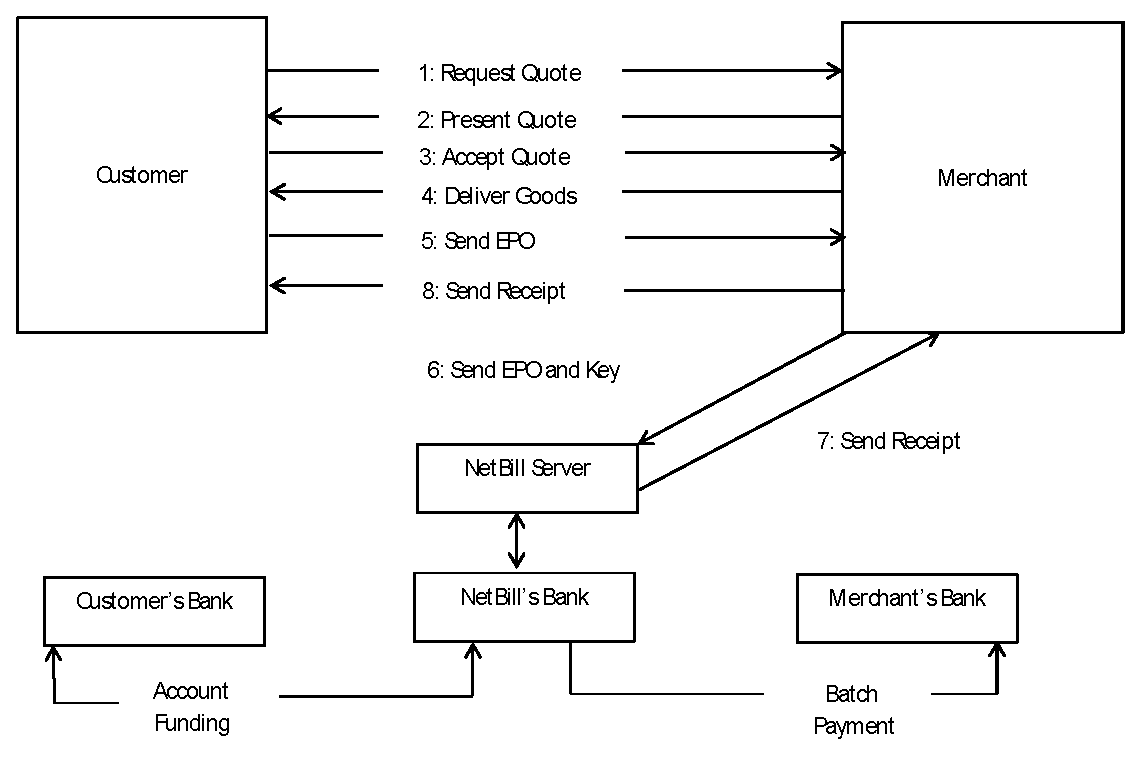
\includegraphics[width=12cm, height=8cm]{figures/figure1.eps}
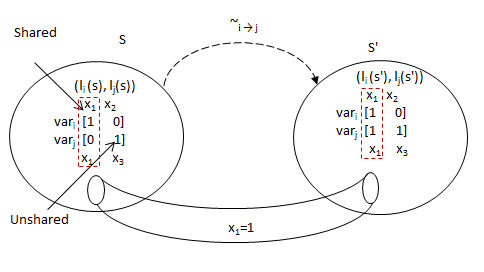
\includegraphics[width=.70 \columnwidth]{figures/figure8.png}
%%\includegraphics[scale=0.5]{figure1}
\caption{The NetBill payment protocol} \label{figure8}
\end{figure}

\end{frame}

%%%%%%%%%%%%%%%%%%%%%%%%%%%%%%%% frame15 outline page

%%%%%%%%%%%%%%%%%%%%%%%%%%%%%%%%%%%%%%%%%%%%%%%%%%%%%%%%%%%%%%%%%%%%%%%%%%%%%%
\begin{frame}{Computation Tree Logic of Knowledge (CTLK)}
\begin{definition} [Model of CTLK]\label{Model of CTLK}
A model $ \mathcal{M_K}$ $=(S,I,R_t,\{\approx_i|i\in \mathcal{ A}\}, \mathcal{V})$ that belongs to the set of all models $\mathbb{M}$ is a tuple, where:
\begin {itemize}
\item $ S \subseteq L_1 \times \dots \times L_n $ is the set of
reachable global states for the system.
\item $ I \subseteq S $ is a set of initial global states for the system.
\item $ R_t \subseteq S \times S $ is the transition relation defined by $( s,s') \in R_t $ iff there exists a joint action $( a_1, \dots , a_n) \in ACT $ such that $ \tau (s, a_1, \dots, a_n) = s'$.
\item For each agent $i \in \mathcal{A}$, $ \approx _i  \subseteq S \times S
$ is the epistemic accessibility relation defined by $ s \approx_i
s' $ iff $ l_i(s) = l_i(s') $.
\item $ \mathcal{V} : S \rightarrow 2 ^{\Phi_p} $ is a valuation function where $\Phi_p $ is a set of atomic propositions.
\end {itemize}
\label {dfn: Model of CTLK}
\end{definition}
\end{frame}
%%%%%%%%%%%%%%%%%%%%%%%%%%%%%%%%%%%%%%%%%%%%%%%%%%%%%%%%%%%%%%%%%%%%%%%%%%%%%%%
\begin{frame}{Syntax of CTLK}
\begin{definition} [Syntax of CTLK]\label{Syntax of CTLK}~\\
$~~~~~~~~~~~~~ \varphi ::= p \mid \neg \varphi \mid \varphi \vee
\varphi \mid EX \varphi  \mid E ( \varphi U \varphi) \mid EG
\varphi \mid K_i \varphi$\\
Where:
\begin{itemize}
\item $ p \in \Phi_p$ is an atomic proposition; \item The boolean
connectives $\neg$, and $\vee$ are defined in the usual way; \item
$E$ is the existential quantifier on paths; \item $X$, $U$, and
$G$ are CTL path modal connectives standing for ``next", ``until",
and ``globally" respectively; and \item The modal connective $K_i$
stands for ``knowledge for agent $i$".
\end{itemize}
\label {dfn: Syntax of CTLK}
\end{definition}
In this logic, \textbf{$K_i \varphi$ is read as ``agent $i$ knows
$\varphi"$.}
\end{frame}
%%%%%%%%%%%%%%%%%%%%%%%%%%%%%%%%%%%%%%%%%%%%%%%%%%%%%%%%%%%%%%%%%%%%%%%%%%%%%%
\begin{frame}{Satisfaction of CTLK}
\begin{definition} [Satisfaction of CTLK]~\\
Given the model $ \mathcal M$, the satisfaction of a CTLK formula
$ \varphi$ in a global state $ s$, denoted by $ (\mathcal M, s )
\models \varphi$, is recursively defined as follows:

\begin{itemize}
\item $ (\mathcal{M}, s ) \models p$ iff $ p \in \mathcal{V}(s)$;
\item $ (\mathcal{M}, s ) \models \neg \varphi$ iff $ (\mathcal{M}, s ) \nvDash \varphi$;
\item $ (\mathcal{M}, s ) \models \varphi \vee \psi$ iff $(\mathcal{M}, s ) \models \varphi$ or $(\mathcal{M}, s ) \models \psi$;
\item $ (\mathcal{M}, s ) \models EX \varphi $ iff there exists a path $\pi$ starting at $s$ such that $ (\mathcal{M}, \pi(1) ) \models \varphi$;
\item $ (\mathcal{M}, s ) \models E ( \varphi U \psi)$ iff there exists a path $\pi$ starting at $s$ such that for some $ k \geq 0$,
$ (\mathcal{M}, \pi(k) ) \models \psi$ and $ (\mathcal{M}, \pi(j) ) \models \varphi$ for all $ 0 \leq j < k$;

\end{itemize}
\label {dfn: Satisfaction of CTLK}
\end{definition}
\end{frame}
%%%%%%%%%%%%%%%%%%%%%%%%%%%%%%%%%%%%%%%%%%%%%%%%%%%%%%%%%%%%%%%%%%%%%%%%%%
\begin{frame}{Satisfaction of CTLK}
\begin{definition} [Satisfaction of CTLK]~\\
\begin{itemize}
\item $ (\mathcal{M}, s ) \models EG \varphi$ iff there exists a path $\pi$  starting at $s$ such that $ (\mathcal{M}, \pi(k) ) \models \varphi$ for all $ k \geq 0$;
\item $ (\mathcal{M}, s ) \models K_i \varphi $ iff for all global states $s' \in S$ such that $s \approx_i s'$, we have $(\mathcal{M}, s' ) \models \varphi $.
\end{itemize}
\label {dfn: Satisfaction of CTLK}
\end{definition}
\end{frame}
%%%%%%%%%%%%%%%%%%%%%%%%%%%%%%%%%%%%%%%%%%%%%%%%%%%%%%%%%%%%%%%%%%%%%%%%%%%%%
\begin{frame}{Computation Tree Logic of Commitment (CTLC)}
CTLC logic is an extension of CTL logic with modalities for reasoning about \textbf{commitments and their fulfillment}.
\begin{definition} [Model of CTLC]\label{Model of CTLC}
A model $\mathcal{M_C}=(S,I,R_t, \{\sim _{i \rightarrow j}|{(i,j)\in \mathcal{A}^2}\},\mathcal{V})$ that belongs to the set of all models $\mathbb{M}$ is a tuple, where:
\begin {itemize}
\item $S, I, R_t$ and $\mathcal{V}$ are the same as in Definition (Model of CTLK).
\item For each pair $(i, j) \in \mathcal{A}^2 $, $\sim _{i \rightarrow j} \subseteq S \times S $ is the social accessibility relation defined by $ s \sim _{i \rightarrow j} s' $ iff
     1) $ l_i(s) = l_i(s') $ and 2) $ Var_i \cap Var_j \neq \emptyset $ such that  $ \forall x \in Var_i \cap Var_j $ we have $ l_i^x(s) = l_j^x(s') $ and $ \forall y \in Var_j - Var_i $ we have $ l_j^y(s) = l_j^y(s')$.

\end {itemize}
\label {dfn: Model of CTLC}
\end{definition}
\end{frame}
%%%%%%%%%%%%%%%%%%%%%%%%%%%%%%%%%%%%%%%%%%%%%%%%%%%%%%%%%%%%%%%%%%%%%%%%%%%%%%
\begin{frame} {Syntax of CTLC}
\begin{definition}[Syntax of CTLC]~\\
$ ~~~~~~~~~~~~~\varphi ::= p \mid \neg \varphi \mid \varphi \vee
\varphi \mid EX \varphi  \mid E ( \varphi U \varphi) \mid EG
\varphi \mid C_{i\rightarrow j} \varphi \mid Fu (C_{i\rightarrow
j}\varphi)$.
\label {dfn: Syntax of CTLC}\\
Where:
\begin{itemize}
  \item $ p, E, X, G, U, \neg $ and $\vee$ are defined as in Definition (Syntax of CTLK);
  \item The modal connective $C_{i \rightarrow j}$ stands for ``commitment from $i$ to $j$"; and
  \item The modal connective $Fu$ stands for ``fulfillment".
\end{itemize}
\end{definition}
\textbf{In this logic, $C_{i\rightarrow j}\varphi$ is read as ``agent $i$ commits towards agent $j$ to bring about $\varphi$". $Fu (C_{i\rightarrow j}\varphi)$ is read as ``the commitment $C_{i\rightarrow j}\varphi$ is fulfilled".}
\end{frame}
%%%%%%%%%%%%%%%%%%%%%%%%%%%%%%%%%%%%%%%%%%%%%%%%%%%%%%%%%%%%%%%%%%%%%%%%%%%%%%
\begin{frame} {Satisfaction of CTLC}
As the main fragment of CTLC logic is the CTL logic, hereafter, we only recall the semantics of the commitment and fulfillment modalities.
\begin{itemize}
\item $ (\mathcal{M_C}, s ) \models C_{i\rightarrow j} \varphi $ iff for all global states $ s' \in S $ such that $ s \sim_{i \rightarrow j} s' $, we have $ (\mathcal{M_C}, s' ) \models \varphi $;
\item $ (\mathcal{M_C}, s ) \models Fu (C_{i\rightarrow j} \varphi)$ iff there exists $ s' \in S $ such that $ s' \sim_{i \rightarrow j} s $ and $ (\mathcal{M_C}, s' ) \models C_{i\rightarrow j} \varphi$.
\end{itemize}
\end{frame}
%%%%%%%%%%%%%%%%%%%%%%%%%%%%%%%%%%%%%%%%%%%%%%%%%%%%%%%%%%%%%%%%%%%%%%%%%%%%%%%
%%%%%%%%%%%%%%%%%%%%%%%%%%%%%%%%%%%%%%%%%%%%%%%%%%%%%%%%%%%%%%%%%%%%%%%%%%%%%%%
\section{Proposed Research}
\begin{frame}{Presentation Outline}
    \begin{itemize}
     	\itemsep=.5cm
    	\item Introduction
    	\item Background and Literature Review
    	\item {\bf Proposed Research}
        \item Contribution and Research Activities
    	\item Time Line
    \end{itemize}
\end{frame}

%%%%%%%%%%%%%%%%%%%%%%%%%%%%%%%% frame16 Proposed Research %%%%%%%%%%%%%%%%%%%%%%%%%%%%%%%%%%%%%
%%%%%%%%%%%%%%%%%%%%%%%%%%%%%%%%%%%%%%%%%%%%%%%%%%%%%%%%%%%%%%%%%%%%%%%%%%%%%%%
\subsection{Combining Logics}

\begin{frame}{A schematic view of our approach}

\begin{figure}[htbp]
\centering
%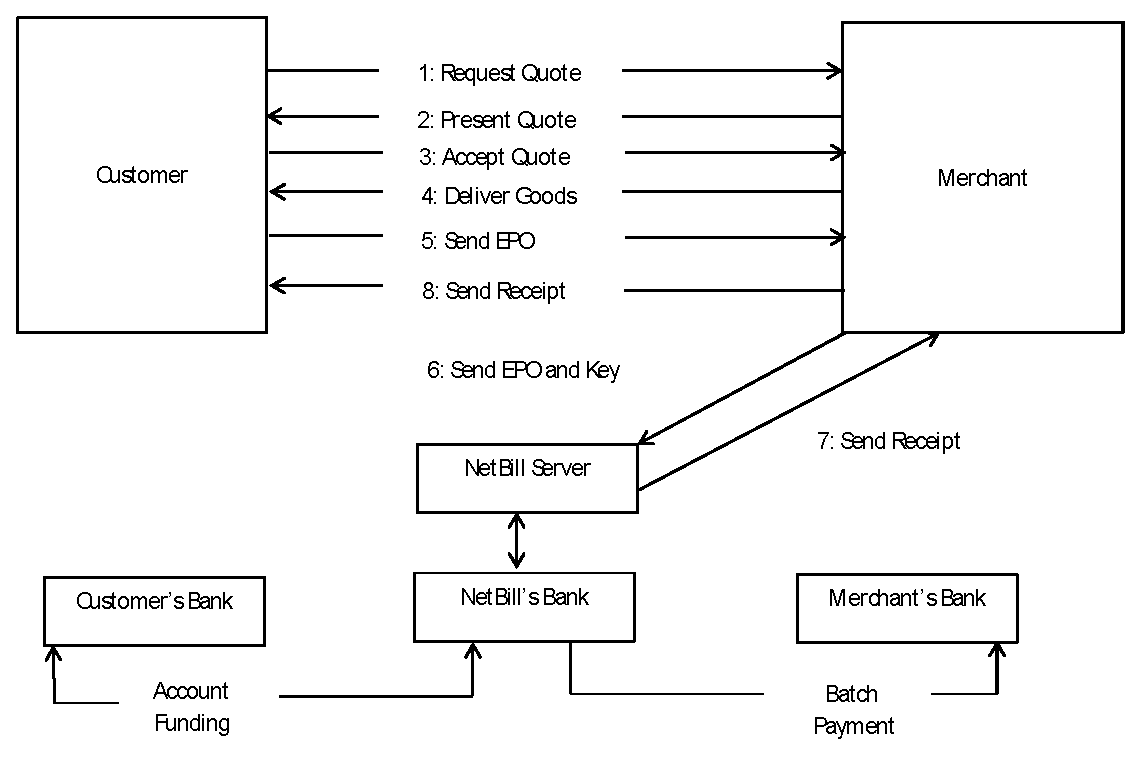
\includegraphics[width=12cm, height=8cm]{figures/figure1.eps}
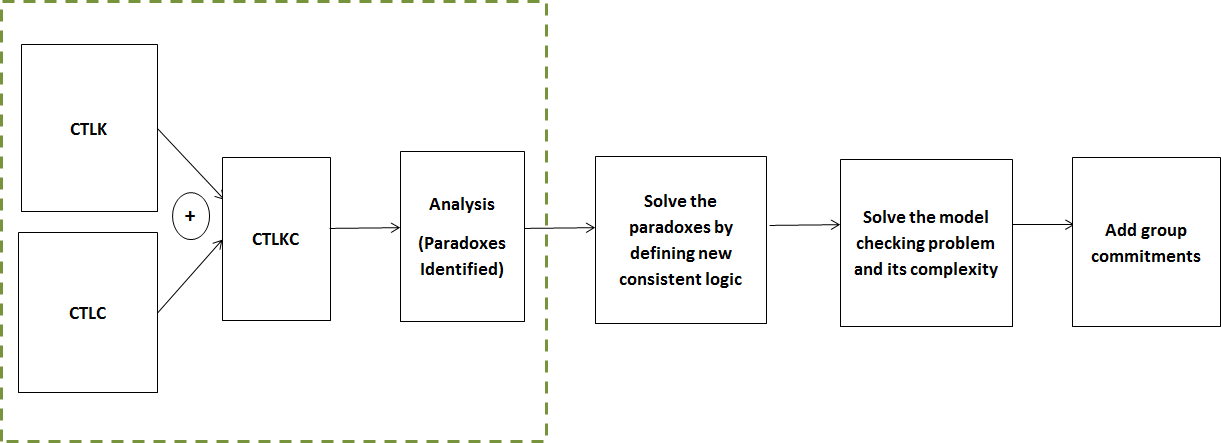
\includegraphics[width=1.05 \columnwidth]{figures/figure9.png}
%%\includegraphics[scale=0.5]{figure1}
%\caption{Our approach} %\label{figure9}
\end{figure}

\end{frame}

%%%%%%%%%%%%%%%%%%%%%%%%%%%%%%%%%%%%%%%%%%%%%%%%%%%%%%%%%%%%%%%%%%%%%%%%%%%%%%%
    \begin{frame}{Combining Logics}
Given \textbf{two logics} $L_1$ and $L_2$, their \textbf{languages} $\mathcal{L}_1$ and $\mathcal{L}_2$, and their
\textbf{axiomatic systems} $\mathcal{X}_1$ and $\mathcal{X}_2$, the logic
$L_1 \otimes L_2$ is the smallest logic with the following
characteristics:
\begin{itemize}
  \item The language $\mathcal{L}_{L_1\otimes L_2}$ is the union of $\mathcal{L}_{L_1}$ and $\mathcal{L}_{L_2}$.
  \item The logic $L_1 \otimes L_2$ is axiomatised by the set of axioms $\mathcal{X}_1 \cup \mathcal{X}_2$.
\end{itemize}
If the logics $L_1$ and $L_2$ are interpreted using Kripke frames
$F_1 = (S, R_1^1, \dots, R_n^1)$ and $F_2 = (S, R_1^2, \dots
,R_m^2 )$ where $R^1_{x/x\in[1,n]}$ and $R^2_{y/y\in[1,m]}$ are
\textbf{accessibility relations}, then the semantics for $L_1 \otimes L_2$
can be defined in the Kripke frame $F =(S, R_1^1, \dots , R_n^1,
R_1^2, \dots ,R_m^2 )$ obtained by the \textit{independent join} of the two
frames $F_1$ and $F_2$.
    \end{frame}

%%%%%%%%%%%%%%%%%%%%%%%%%%%%%%%% frame17 Proposed Research
\begin{frame} {Model of CTLKC}
\begin{definition} [Model of CTLKC]\label{Model of CTLKC}
A model $\mathcal{M}=(S,I,R_t,\{\approx_i|i\in \mathcal{ A}\},\{\sim _{i \rightarrow j}|{(i,j)\in \mathcal{A}^2}\},\mathcal{V})$ that belongs to the set of all models $\mathbb{M}$ is a tuple, where:
\begin {itemize}
\item $S, I, R_t$ and $\mathcal{V}$ are the same as in Definition (Model of CTLK);
\item For each agent $i \in \mathcal{A}$, $ \approx _i  \subseteq S \times S
$ is the epistemic accessibility relation defined by $ s \approx_i
s' $ iff $ l_i(s) = l_i(s') $;
\item For each pair $(i, j) \in \mathcal{A}^2 $, $\sim _{i \rightarrow j} \subseteq S \times S $ is the social accessibility relation defined by $ s \sim _{i \rightarrow j} s' $ iff
     1) $ l_i(s) = l_i(s') $ and
     2) $ Var_i \cap Var_j \neq \emptyset $ such that  $ \forall x \in Var_i \cap Var_j $ we have $ l_i^x(s) = l_j^x(s') $ and $ \forall y \in Var_j - Var_i $ we have $ l_j^y(s) = l_j^y(s')$;
\item $ \mathcal{V} : S \rightarrow 2 ^{\Phi_p} $ is a valuation function where $\Phi_p $ is a set of atomic propositions.
\end {itemize}
\label {dfn: Model of CTLKC}
\end{definition}
 \end{frame}
%%%%%%%%%%%%%%%%%%%%%%%%%%%%%%%%%%%%%%%%%%%%%%%%%%%%%%%%%%%%%%%%%%%%%%%%%%%%%%%
\begin{frame} {Syntax of CTLKC}

\begin{definition}[Syntax of CTLKC]~\\
$ ~~~~~~~~~~~~~\varphi ::= p \mid \neg \varphi \mid \varphi \vee
\varphi \mid EX \varphi  \mid E ( \varphi U \varphi) \mid EG
\varphi\mid K_i \varphi \mid C_{i\rightarrow j} \varphi \mid Fu
(C_{i\rightarrow j}\varphi)$. \label {dfn: Syntax of CTLKC}
\end{definition}

\end{frame}


%%%%%%%%%%%%%%%%%%%%%%%%%%%%%%%% frame18 Proposed Research %%%%%%%%%%%%%%%%%%%%%%%%%%%%%%%%%%%%%%%%%%%%%%%%%%%%%%%%%%%%%%%%%%%%%%%%%%%%%%%
\begin{frame}{Selection Criteria}
We propose the following criteria based on \textbf{common intuitions}:
\begin{itemize}
%\begin{enumerate}
  \item It should not be the case that an agent commits about everything he knows to others.
  \item It should not be the case that an agent commits about everything known by others.
  \item An agent should know about his own commitment.
  \item An agent should be aware of any commitment directed towards him.
  \item An agent should know the content of his fulfilled commitment.
  \item An agent should know the content of any fulfilled commitment directed towards him.


\end{itemize}

\end{frame}
%%%%%%%%%%%%%%%%%%%%%%%%%%%%%%%%%%%%%%%%%%%%%%%%%%%%%%%%%%%%%%%%%%%%%%%%%%%%%%%
\begin{frame}{Continue: Selection Criteria}
\begin{itemize}
 \item An agent should know about the fulfillment of his commitment.
 \item An agent should know about the fulfillment of any commitment directed towards him.
  \item A sincere agent should know (i.e., believe) the content of his own commitment.
  \item A sincere agent should fulfill his commitment.
  \item A liar agent could not know (i.e., believe) the content of his commitment.
  \item If an agent knows about his own commitment, then this commitment should exist, which means an agent should not know about a non-existing commitment.
\end{itemize}
%\end{enumerate}
\end{frame}

%%%%%%%%%%%%%%%%%%%%%%%%%%%%%%%%%%%%%%%%%%%%%%%%%%%%%%%%%%%%%%%%%%%%%%%%%%%%%%

\begin{frame}{Running Example: NetBill Payment Protocol}
%
\begin{figure}[htbp]
\centering
%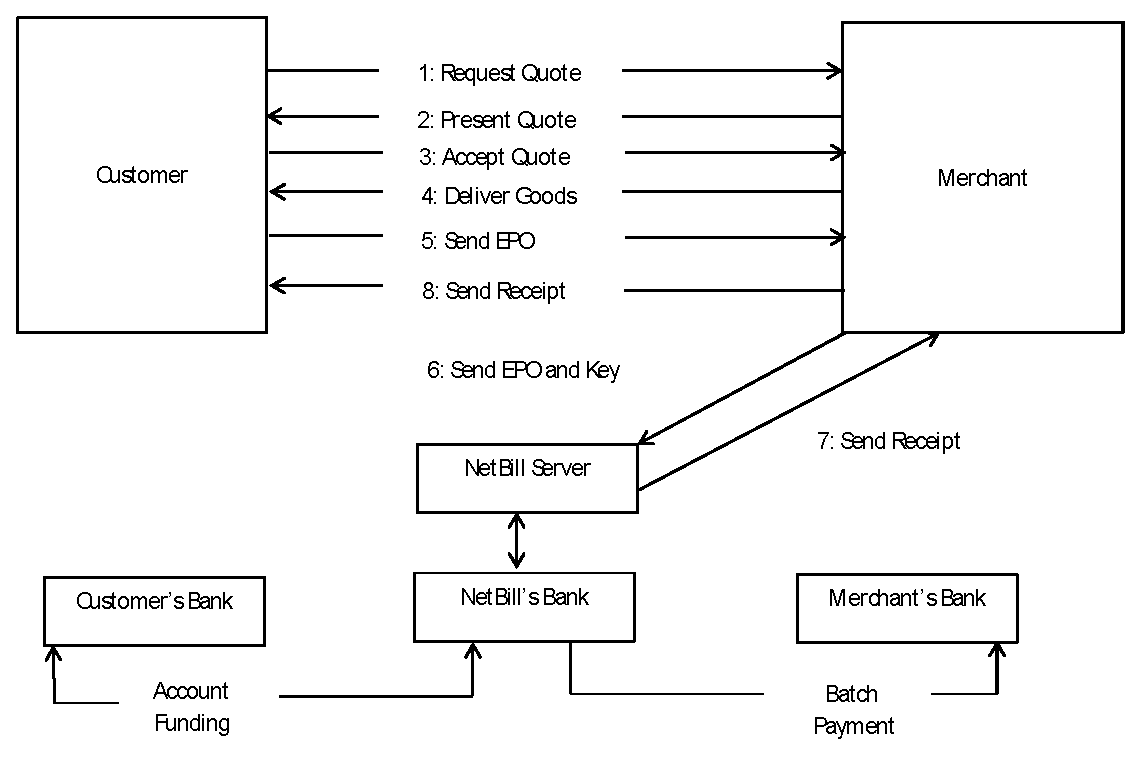
\includegraphics[width=12cm, height=8cm]{figures/figure1.eps}
\includegraphics[width=.75 \columnwidth]{figures/figure1.png}
%%\includegraphics[scale=0.5]{figure1}
%\caption{The NetBill payment protocol} \label{figure1}
\end{figure}
\begin{itemize}
\item $C_{Cus \rightarrow Mer}$ $sendPayment$.
 \item $C_{Mer \rightarrow Cus}$ $deliverGoods$.
 \end{itemize}
\end{frame}

%%%%%%%%%%%%%%%%%%%%%%%%%%%%%%%% frame19 Proposed Research
%%%%%%%%%%%%%%%%%%%%%%%%%%%%%%%%%%%%%%%%%%%%%%%%%%%%%%%%%%%%%%%%%%%%%%%%%%%%%%%
\subsection{Desiderata of Paradoxes}

\begin{frame}{Desiderata of Paradoxes}
Paradoxes are represented as reasoning rules that are: 1) not reasonable in
open MAS, but they are valid in CTLKC; or 2) desirable for the
interaction between knowledge and commitments, but they can get
violated in CTLKC because they are not valid.
 \begin{enumerate}

\vspace{0.2cm} \item [P1.]\textbf{[Committing everything known to
others]}

$K_i \varphi \Rightarrow C_{i \rightarrow j}\varphi, $ for all $j
\in A$ where $i \neq j$.

\textbf{ Meaning:} An agent (the debtor) commits towards all other
agents (the creditors) about what he knows.\\
\textbf{Example 1:}
$K_{Mer}$ $deliverGoods \Rightarrow$ $C_{Mer \rightarrow
Cus}$ $deliverGoods$.

\vspace{0.2cm} \item [P2.]\textbf{[Committing everything known by
others]}

 $ K_i K_j \varphi \Rightarrow C_{i \rightarrow j} \varphi$ such that $ i \neq j$.

\textbf{Meaning:} An agent (the debtor) commits toward another
agent (the creditor) to bring about what he (i.e., the debtor)
knows about the creditor's knowledge.\\
\textbf{Example 2:}
$K_{Cus} K_{Mer}$ $deliverGoods \Rightarrow$ $C_{Cus \rightarrow Mer}$
$deliverGoods$.


\end{enumerate}
       	
\end{frame}
%%%%%%%%%%%%%%%%%%%%%%%%%%%%%%%% frame20 Proposed Research %%%%%%%%%%%%%%%%%%%%%%%%%%%%%%%%%%%%%

\begin{frame}{Continue: Desiderata of Paradoxes}
 \begin{enumerate}
\vspace{0.2cm} \item [P3.][\textbf{Committing everything known
from others}]
$ K_i K_j \varphi \Rightarrow C_{j \rightarrow i} \varphi$ such that $ i \neq j$.

\textbf{Meaning:} An agent (the debtor) commits toward another
agent (the creditor) to bring about what the creditor knows about
the debtor's knowledge.\\
\textbf{Example 3:}\\
$K_{Cus} K_{Mer}$ $deliverGoods \Rightarrow$ $C_{Mer \rightarrow Cus}$
$deliverGoods$.

\vspace{0.2cm} \item [P4.][\textbf{Knowing about his own
commitment}]

$C_{i\rightarrow j} \varphi \Rightarrow K_i (C_{i\rightarrow j}
\varphi) $ where $i \neq j$.

\textbf{Meaning:} An agent knows about his commitment.


\textbf{Example 4:}\\
$C_{Cus \rightarrow Mer}$ $sendPayment $ $\Rightarrow K_{Cus}$ $(C_{Cus \rightarrow Mer}$ $sendPayment)$.
\end{enumerate}

        	
\end{frame}
%%%%%%%%%%%%%%%%%%%%%%%%%%%%%%%%%%%%%%%%%%%%%%%%%%%%%%%%%%%%%%%%%%%%%%%%%%%%%%%

%%%%%%%%%%%%%%%%%%%%%%%%%%%%%%%%%%%%%%%%%%%%%%%%%%%%%%%%%%%%%%%%%%%%%%%%%%%%%%%

\begin{frame}{Continue: Desiderata of Paradoxes}

\begin{figure}[htbp]
    \begin{center}
%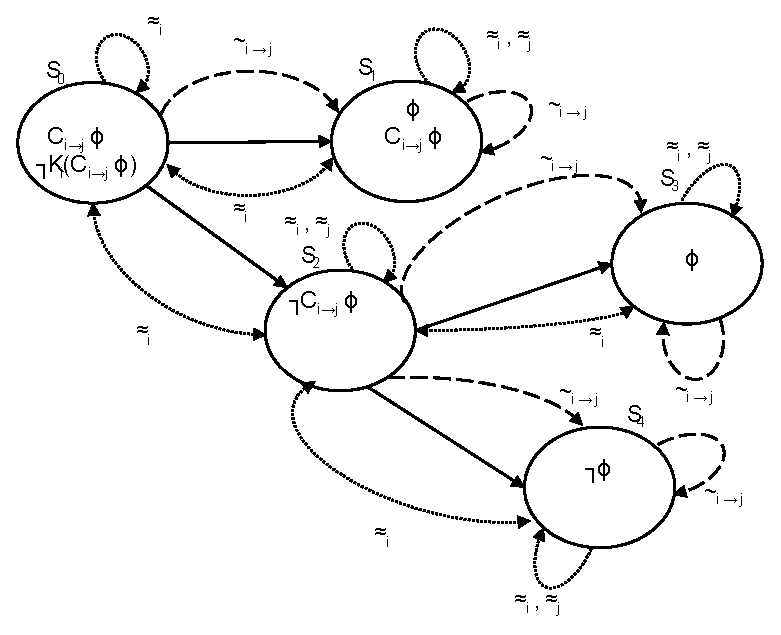
\includegraphics[width=10cm, height=5cm]{figures/figure2.eps}
    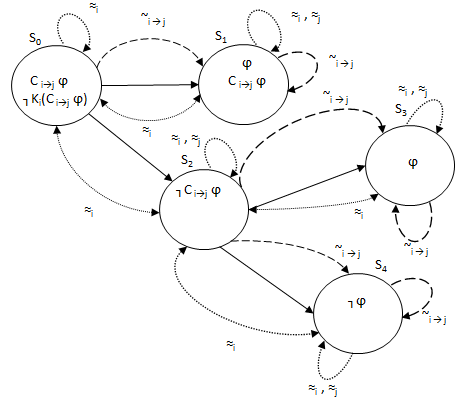
\includegraphics[width=.75 \columnwidth]{figures/figure2.png}
   % \caption{Model 1} \label{figure2}
    \end{center}
    \end{figure}
\end{frame}
%%%%%%%%%%%%%%%%%%%%%%%%%%%%%%%%%%%%%%%%%%%%%%%%%%%%%%%%%%%%%%%%%%%%%%%%%%%%%%%

\begin{frame}{Continue: Desiderata of Paradoxes}
\begin{enumerate}
\vspace{0.2cm} \item [P5.][\textbf{Knowing the content of his own
fulfilled commitment}]

$Fu (C _{i\rightarrow j} \varphi) \Rightarrow K _i \varphi$ where
$i \neq j$.

\textbf{Meaning:} An agent knows the content of his fulfilled
commitment.\\
\textbf{Example 5:}\\
$Fu (C _{Cus\rightarrow Mer} sendPayment) \Rightarrow K_{Cus}$ $sendPayment$.
\begin{figure}[htbp]
    \begin{center}
%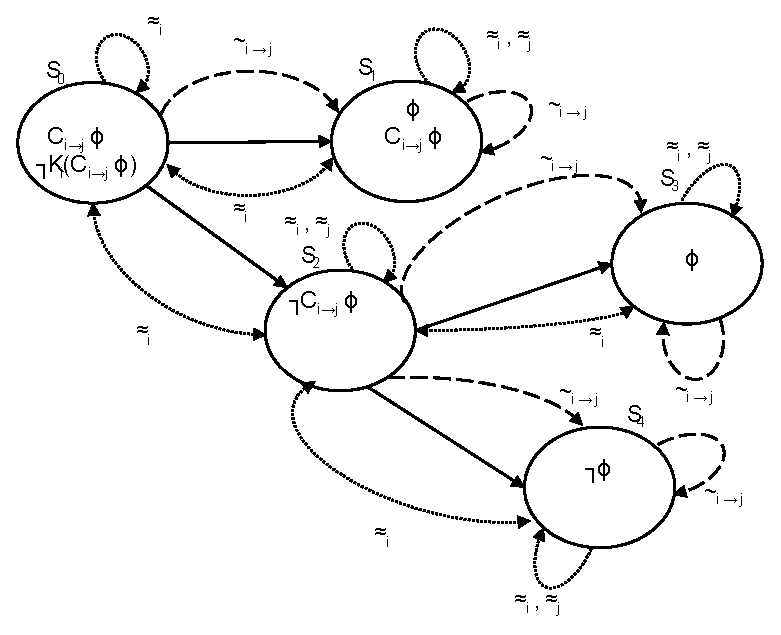
\includegraphics[width=10cm, height=5cm]{figures/figure2.eps}
    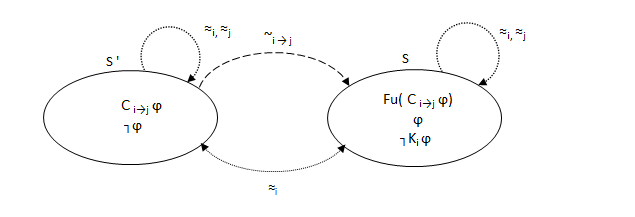
\includegraphics[width=.75 \columnwidth]{figures/figure3.png}
   % \caption{Model 2} \label{figure3}
    \end{center}
    \end{figure}

\end{enumerate}     	
\end{frame}
%%%%%%%%%%%%%%%%%%%%%%%%%%%%%%%% frame23 Proposed Research %%%%%%%%%%%%%%%%%%%%%%%%%%%%%%%%%%%%%
%%%%%%%%%%%%%%%%%%%%%%%%%%%%%%%%%%%%%%%%%%%%%%%%%%%%%%%%%%%%%%%%%%%%%%%%%%%%%%%

 \begin{frame}{Continue: Desiderata of Paradoxes}
 \begin{enumerate}

\vspace{0.2cm} \item [P6.][\textbf{Knowing the content of the
other's fulfilled commitment}]

$Fu (C _{i\rightarrow j} \varphi) \Rightarrow K_j \varphi$ where
$i \neq j$.

\textbf{Meaning:} The creditor knows the content of the debtor's
fulfilled commitment.\\
\textbf{Example 6:}\\
$ Fu (C_{cust \rightarrow Mer}$ $sendPayment)$ $\Rightarrow $ $k_{Mer} sendPayment$.
	\begin{figure}[htbp]
\begin{center}
%\includegraphics[width=12cm, height=5cm]{figures/figure4.eps}
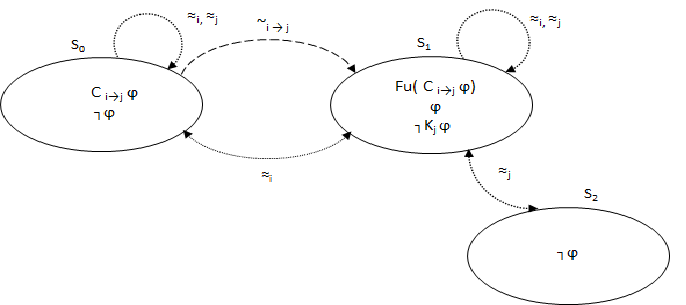
\includegraphics[width=.70 \columnwidth]{figures/figure4.png}
%\caption{Model 3} \label{figure4}
\end{center}
\end{figure}
\end{enumerate}
\end{frame}

%%%%%%%%%%%%%%%%%%%%%%%%%%%%%%%% frame24 Proposed Research %%%%%%%%%%%%%%%%%%%%%%%%%%%%%%%%%%%%%
%%%%%%%%%%%%%%%%%%%%%%%%%%%%%%%%%%%%%%%%%%%%%%%%%%%%%%%%%%%%%%%%%%%%%%%%%%%%%%
\begin{frame}{Continue: Desiderata of Paradoxes}
\begin{enumerate}
    \vspace{0.2cm} \item [P7.][\textbf{Knowing the commitment of the
other}]

$C_{i\rightarrow j} \varphi \Rightarrow AF K_j (C_{i\rightarrow j}
\varphi) $ where $i \neq j$.

\textbf{Meaning:} An agent should be aware of any commitments
directed towards him.\\
\textbf{Example 7:}\\
$C_{Mer \rightarrow Cus}$ $deliverGoods$ $\Rightarrow $ $AF K_{Cus}(C_{Mer \rightarrow Cus}$
$deliverGoods$).
\begin{figure}[htbp]
\centering
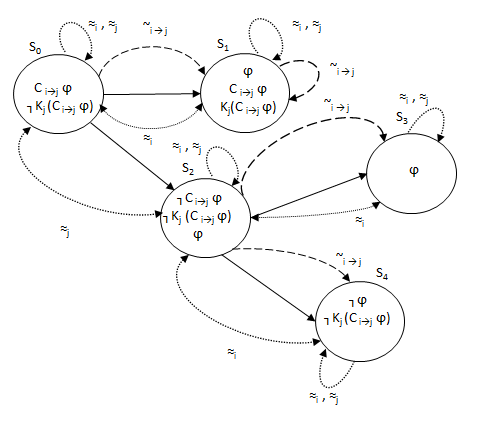
\includegraphics[width=.50 \columnwidth]{figures/figure5.png}
%\includegraphics[width=12cm, height=7cm]{figures/figure5.eps}
%\includegraphics[scale=0.5]{figure4.eps}
%\caption{Model 4} \label{figure5}
\end{figure}

\end{enumerate}
\end{frame}
%%%%%%%%%%%%%%%%%%%%%%%%%%%%%%%%%%%%%%%%%%%%%%%%%%%%%%%%%%%%%%%%%%%%%%%%%%%%%%%
\begin{frame}{Continue: Desiderata of Paradoxes}
\begin{enumerate}
    \vspace{0.2cm} \item [P8.][\textbf{Knowing the fulfillment of his
own commitment}]

$Fu(C _{i\rightarrow j} \varphi) \Rightarrow K_i Fu(C
_{i\rightarrow j} \varphi)$ where $i \neq j$.

\textbf{Meaning:} The agent knows that he fulfills his commitment.\\
\textbf{Example 8:}\\
$Fu(C_{Cus\rightarrow Mer} sendPayment)\Rightarrow K_{Cus}Fu(C_{Cus \rightarrow Mer} sendPayment)$.

\vspace{0.2cm} \item [P9.][\textbf{Knowing the fulfillment of the
debtor's commitment}]


$Fu(C _{i\rightarrow j} \varphi) \Rightarrow K_j Fu(C_{i\rightarrow j} \varphi)$ where $i \neq j$.

\textbf{Meaning:} The creditor knows that the debtor fulfills his
commitment.\\
\textbf{Example 9:}\\
$Fu(C_{Cus \rightarrow Mer} sendPayment)\Rightarrow K_{Mer} Fu(C_{Cus \rightarrow Mer} sendPayment)$.
\end{enumerate}
\end{frame}
%%%%%%%%%%%%%%%%%%%%%%%%%%%%%%%% frame25 outline page %%%%%%%%%%%%%%%%%%%%%%%%%%%%%%%%%%%%%
%%%%%%%%%%%%%%%%%%%%%%%%%%%%%%%%%%%%%%%%%%%%%%%%%%%%%%%%%%%%%%%%%%%%%%%%%%%%%%%
\subsection{CTLKC properties}
\begin{frame}{CTLKC properties}
In addition to the properties of knowledge (in CTLK) and commitments (in CTLC), those properties hold in CTLKC:
\begin{enumerate}

\vspace{0.2cm} \item [Prop 1.] $C_{i \rightarrow j}\varphi
\Rightarrow \varphi$ is satisfiable but not valid.
\vspace{0.2cm} \item [Prop 2.] $C_{i \rightarrow j}\varphi
\Rightarrow K_i \varphi$ is satisfiable but not valid.
\vspace{0.2cm} \item [Prop 3.] $(C_{i \rightarrow j}\varphi \wedge
K_i (\varphi \Rightarrow \psi)) \Rightarrow C_{i \rightarrow j}
\psi$ is valid.
\vspace{0.2cm} \item [Prop 4.] $(C_{i \rightarrow j}(\varphi
\Rightarrow \psi) \wedge K_i \varphi) \Rightarrow C_{i \rightarrow
j} \psi$ is valid.
\vspace{0.2cm} \item [Prop 5.] $(C_{i \rightarrow j}\varphi \wedge
K_j (\varphi \Rightarrow \psi)) \Rightarrow C_{i \rightarrow j}
\psi$ is satisfiable but not valid.
\vspace{0.2cm} \item [Prop 6.] $(C_{i \rightarrow j}(\varphi
\Rightarrow \psi) \wedge K_j \varphi) \Rightarrow C_{i \rightarrow
j} \psi$ is satisfiable but not valid

\end{enumerate}
\end{frame}

\section{Research Activities}
\begin{frame}{Contribution and Research Activities}
    \begin{itemize}
     	\itemsep=.5cm
    	\item Introduction
    	\item Background and Literature Review
    	\item Proposed Research
        \item {\bf Contribution and Research Activities}
    	\item Time Line
    \end{itemize}
\end{frame}

%%%%%%%%%%%%%%%%%%%%%%%%%%%%%%%% frame26 Contribution and Research Activities %%%%%%%%%%%%%%%%%%%%%%%%%%%%%%%%%%%%%
%%%%%%%%%%%%%%%%%%%%%%%%%%%%%%%%%%%%%%%%%%%%%%%%%%%%%%%%%%%%%%%%%%%%%%%%%%%%%%
\subsection{Contributions}
    \begin{frame}{Contributions}

    \begin{itemize}
     \itemsep=.35cm
     \item A new combined temporal logic, called CTLKC, that combines both CTLK and CTLC logics is introduced.
     \item This logic served as a language to express a set of rules that are used to reason about the interaction between knowledge and social commitments.
     \item Selection criteria are proposed to capture such reasoning rules.
     \item Nine paradoxes are recognized in CTLKC logic that should be addressed in any consistent logic combining knowledge and commitments.
     \item Six properties are identified and should be met in any logic combining knowledge and commitments.
        \end{itemize}


    \end{frame}
%%%%%%%%%%%%%%%%%%%%%%%%%%%%%%%% frame27 Contribution and Research Activities



%%%%%%%%%%%%%%%%%%%%%%%%%%%%%%%% frame30 outline page
%%%%%%%%%%%%%%%%%%%%%%%%%%%%%%%%%%%%%%%%%%%%%%%%%%%%%%%%%%%%%%%%%%%%%%%%%%%%%%%
\section{Milestones}
\begin{frame}{Milestones}
    \begin{itemize}
     	\itemsep=.5cm
    	\item Introduction
    	\item Background and Literature Review
    	\item Proposed Research
        \item Contribution and Research Activities
    	\item {\bf Time Line}
    \end{itemize}
\end{frame}

%%%%%%%%%%%%%%%%%%%%%%%%%%%%%%%%%%%%%%%%%%%%%%%%%%%%%%%%%%%%%%%%%%%%%%%%%%%%%%
\subsection{Research Activities Goal}
    \begin{frame}{Research Activities Goal}
    We aim to cover all possible relations between knowledge and commitments as single and group interactions by:

        \begin{itemize}
              \item Defining a new consistent logic that combines knowledge and commitments and solves the nine paradoxes while satisfying the six properties.
              \item Addressing the model checking problem of the new logic from both algorithmic and complexity perspectives.
              \item Implementing the new model checking algorithms on top of MCMAS+.
              \item Identifying a new semantics for group committing.
              \item Adding the group knowledge to the framework.
        \end{itemize}


\end{frame}

%%%%%%%%%%%%%%%%%%%%%%%%%%%%%%%%
%%%%%%%%%%%%%%%%%%%%%%%%%%%%%%%%%%%%%%%%%%%%%%%%%%%%%%%%%%%%%%%%%%%%%%%%%%%%%%%
\subsection{Time Line}
    \begin{frame}{Time Line}


\begin{figure}[htbp]
\begin{center}
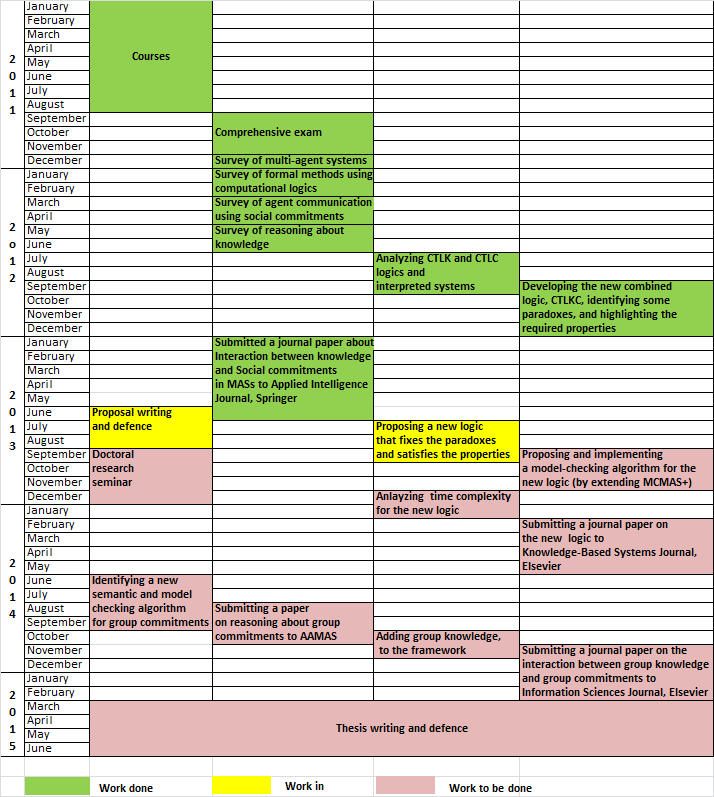
\includegraphics[width=.65 \columnwidth]{figures/figure6.png}
%\includegraphics[width=16cm, height=21cm]{figures/figure6.eps}
%\caption{Schedule time of research} \label{figure6}
\end{center}
\end{figure}
    \end{frame}
%%%%%%%%%%%%%%%%%%%%%%%%%%%%%%%% frame27 Milestones %%%%%%%%%%%%%%%%%%%%%%%%%%%%%%%%%%%%%
%%%%%%%%%%%%%%%%%%%%%%%%%%%%%%%%%%%%%%%%%%%%%%%%%%%%%%%%%%%%%%%%%%%%%%%%%%%%%%%
%%%%%%%%%%%%%%%%%%%%%%%%%%%%%%%%%%%%
%%%%%%%%%%%%%%%%%%%%%%%%%%%%%%%%%%%%%%%%%%%%%%%%%%%%%%%%%%%%%%%%%%%%%%%%%%%%%%
\begin{frame}{Publications}

1- Submitted a journal paper entitled ``\textbf{Interaction between knowledge and Social Commitments in MASs}", Applied Intelligence Journal, Springer.\\

%\centering
%\begin{itemize}
%\item \textbf{Questions Please !}
%\end{itemize}

\end{frame}

\end{document}
